%%%%%%%%%%%%%%%%%%%%%%%%%%%%%%%%%%%%%%%%%
% Wenneker Article
% LaTeX Template
% Version 2.0 (28/2/17)
%
% This template was downloaded from:
% http://www.LaTeXTemplates.com
%
% Authors:
% Vel (vel@LaTeXTemplates.com)
% Frits Wenneker
%
% License:
% CC BY-NC-SA 3.0 (http://creativecommons.org/licenses/by-nc-sa/3.0/)
%
%%%%%%%%%%%%%%%%%%%%%%%%%%%%%%%%%%%%%%%%%

%----------------------------------------------------------------------------------------
%	PACKAGES AND OTHER DOCUMENT CONFIGURATIONS
%----------------------------------------------------------------------------------------

\documentclass[10pt, a4paper, twocolumn]{article} % 10pt font size (11 and 12 also possible), A4 paper (letterpaper for US letter) and two column layout (remove for one column)

%%%%%%%%%%%%%%%%%%%%%%%%%%%%%%%%%%%%%%%%%
% Wenneker Article
% Structure Specification File
% Version 1.0 (28/2/17)
%
% This file originates from:
% http://www.LaTeXTemplates.com
%
% Authors:
% Frits Wenneker
% Vel (vel@LaTeXTemplates.com)
%
% License:
% CC BY-NC-SA 3.0 (http://creativecommons.org/licenses/by-nc-sa/3.0/)
%
%%%%%%%%%%%%%%%%%%%%%%%%%%%%%%%%%%%%%%%%%

%----------------------------------------------------------------------------------------
%	PACKAGES AND OTHER DOCUMENT CONFIGURATIONS
%----------------------------------------------------------------------------------------

\usepackage[english]{babel} % English language hyphenation

\usepackage{microtype} % Better typography

\usepackage{amsmath,amsfonts,amsthm} % Math packages for equations
\usepackage{hyperref}
\hypersetup{colorlinks=true,linkcolor=blue,filecolor=magenta,urlcolor=cyan,pdftitle={An Example},pdfpagemode=FullScreen,}

\urlstyle{same}

\usepackage{dirtree}

\usepackage[svgnames]{xcolor} % Enabling colors by their 'svgnames'

\usepackage[hang, small, labelfont=bf, up, textfont=it]{caption} % Custom captions under/above tables and figures

\usepackage{booktabs} % Horizontal rules in tables

\usepackage{lastpage} % Used to determine the number of pages in the document (for "Page X of Total")

\usepackage{graphicx} % Required for adding images

\usepackage{enumitem} % Required for customising lists
\setlist{noitemsep} % Remove spacing between bullet/numbered list elements

\usepackage{subfigure}
\usepackage{sectsty} % Enables custom section titles
\allsectionsfont{\usefont{OT1}{phv}{b}{n}} % Change the font of all section commands (Helvetica)

%----------------------------------------------------------------------------------------
%	MARGINS AND SPACING
%----------------------------------------------------------------------------------------

\usepackage{geometry} % Required for adjusting page dimensions

\geometry{
	top=1cm, % Top margin
	bottom=1.5cm, % Bottom margin
	left=2cm, % Left margin
	right=2cm, % Right margin
	includehead, % Include space for a header
	includefoot, % Include space for a footer
	%showframe, % Uncomment to show how the type block is set on the page
}

\setlength{\columnsep}{7mm} % Column separation width

%----------------------------------------------------------------------------------------
%	FONTS
%----------------------------------------------------------------------------------------

\usepackage[T1]{fontenc} % Output font encoding for international characters
\usepackage[utf8]{inputenc} % Required for inputting international characters

\usepackage{XCharter} % Use the XCharter font

%----------------------------------------------------------------------------------------
%	HEADERS AND FOOTERS
%----------------------------------------------------------------------------------------

\usepackage{fancyhdr} % Needed to define custom headers/footers
\pagestyle{fancy} % Enables the custom headers/footers

\renewcommand{\headrulewidth}{0.0pt} % No header rule
\renewcommand{\footrulewidth}{0.4pt} % Thin footer rule

\renewcommand{\sectionmark}[1]{\markboth{#1}{}} % Removes the section number from the header when \leftmark is used

%\nouppercase\leftmark % Add this to one of the lines below if you want a section title in the header/footer

% Headers
\lhead{} % Left header
\chead{\textit{\thetitle}} % Center header - currently printing the article title
\rhead{} % Right header

% Footers
\lfoot{} % Left footer
\cfoot{} % Center footer
\rfoot{\footnotesize Page \thepage\ of \pageref{LastPage}} % Right footer, "Page 1 of 2"

\fancypagestyle{firstpage}{ % Page style for the first page with the title
	\fancyhf{}
	\renewcommand{\footrulewidth}{0pt} % Suppress footer rule
}

%----------------------------------------------------------------------------------------
%	TITLE SECTION
%----------------------------------------------------------------------------------------

\newcommand{\authorstyle}[1]{{\large\usefont{OT1}{phv}{b}{n}\color{DarkRed}#1}} % Authors style (Helvetica)

\newcommand{\institution}[1]{{\footnotesize\usefont{OT1}{phv}{m}{sl}\color{Black}#1}} % Institutions style (Helvetica)

\usepackage{titling} % Allows custom title configuration

\newcommand{\HorRule}{\color{DarkGoldenrod}\rule{\linewidth}{1pt}} % Defines the gold horizontal rule around the title

\pretitle{
	\vspace{-50pt} % Move the entire title section up
	\HorRule\vspace{10pt} % Horizontal rule before the title
	\fontsize{32}{36}\usefont{OT1}{phv}{b}{n}\selectfont % Helvetica
	\color{DarkRed} % Text colour for the title and author(s)
}

\posttitle{\par\vskip 10pt} % Whitespace under the title

\preauthor{} % Anything that will appear before \author is printed

\postauthor{ % Anything that will appear after \author is printed
	\vspace{1pt} % Space before the rule
	\par\HorRule % Horizontal rule after the title
	\vspace{0pt} % Space after the title section
}

%----------------------------------------------------------------------------------------
%	ABSTRACT
%----------------------------------------------------------------------------------------

\usepackage{lettrine} % Package to accentuate the first letter of the text (lettrine)
\usepackage{fix-cm}	% Fixes the height of the lettrine

\newcommand{\initial}[1]{ % Defines the command and style for the lettrine
	\lettrine[lines=3,findent=4pt,nindent=0pt]{% Lettrine takes up 3 lines, the text to the right of it is indented 4pt and further indenting of lines 2+ is stopped
		\color{DarkGoldenrod}% Lettrine colour
		{#1}% The letter
	}{}%
}

\usepackage{xstring} % Required for string manipulation

\newcommand{\lettrineabstract}[1]{
	\StrLeft{#1}{1}[\firstletter] % Capture the first letter of the abstract for the lettrine
	\initial{\firstletter}\textbf{\StrGobbleLeft{#1}{1}} % Print the abstract with the first letter as a lettrine and the rest in bold
}

%----------------------------------------------------------------------------------------
%	BIBLIOGRAPHY
%----------------------------------------------------------------------------------------

\usepackage[backend=bibtex,natbib=true]{biblatex} % Use the bibtex backend with the authoryear citation style (which resembles APA)

\addbibresource{example.bib} % The filename of the bibliography

\usepackage[autostyle=true]{csquotes} % Required to generate language-dependent quotes in the bibliography
 % Specifies the document structure and loads requires packages

%----------------------------------------------------------------------------------------
%	ARTICLE INFORMATION
%----------------------------------------------------------------------------------------

\title{TrackG4PS: A Simulation of the PS modules with cosmic rays} % The article title

\author{
	\authorstyle{Piero Viscone} % Authors
	\newline % Space before institutions
    \institution{University of Pisa}
    \newline
    \newline
    
\includegraphics[width=0.02 \textwidth]{img/github-logo.png}   \href{https://github.com/pviscone/TrackG4}{GitHub repository}\\ %
}

% Example of a one line author/institution relationship
%\author{\newauthor{John Marston} \newinstitution{Universidad Nacional Autónoma de México, Mexico City, Mexico}}

\date{} % Add a date here if you would like one to appear underneath the title block, use \today for the current date, leave empty for no date

%----------------------------------------------------------------------------------------

\begin{document}

\maketitle % Print the title

\thispagestyle{firstpage} % Apply the page style for the first page (no headers and footers)

%----------------------------------------------------------------------------------------
%	ABSTRACT
%----------------------------------------------------------------------------------------

\lettrineabstract{The PS modules are prototypes that will be part of the CMS outer tracker detector during the Run4. These modules are currently being tested in a cryostat acquiring cosmic ray data. This paper presents a simulation of the commissioning with cosmic rays of the PS modules and a toy model for tracking.}

%----------------------------------------------------------------------------------------
%	ARTICLE CONTENTS
%----------------------------------------------------------------------------------------
\section{Introduction}

\begin{figure}[h!]
    \centering
    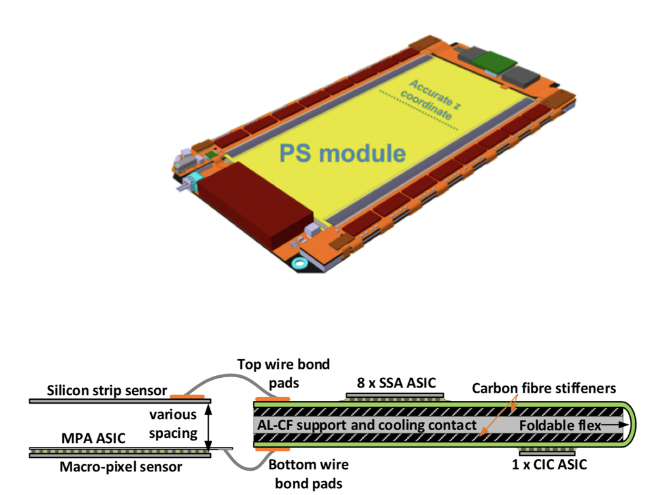
\includegraphics[width=0.48\textwidth]{img/ps_module.png}
    \caption{Assembled PS module (top), front-end sketch (bottom)}
    \label{fig:PS}
\end{figure}
A PS silicon module is made up of one strip sensor with 2 columns of 960 strips with a size of 2.5mm X 0.1 mm and a macro pixel sensor with a matrix of 32 X 960 pixels with a pixel size of 1.5 mm X 0.1 mm. \cite{PS}
\\
\\
The strip sensor and the macro pixel sensor are spaced apart by a variable length, from 1 to 4 mm (in the simulation, this value is set to 4mm).  
\\
\\
These modules are tested with cosmic rays in a cryostat in a grid of 2 columns and 5 layers.
\begin{figure}[h!]
    \centering
    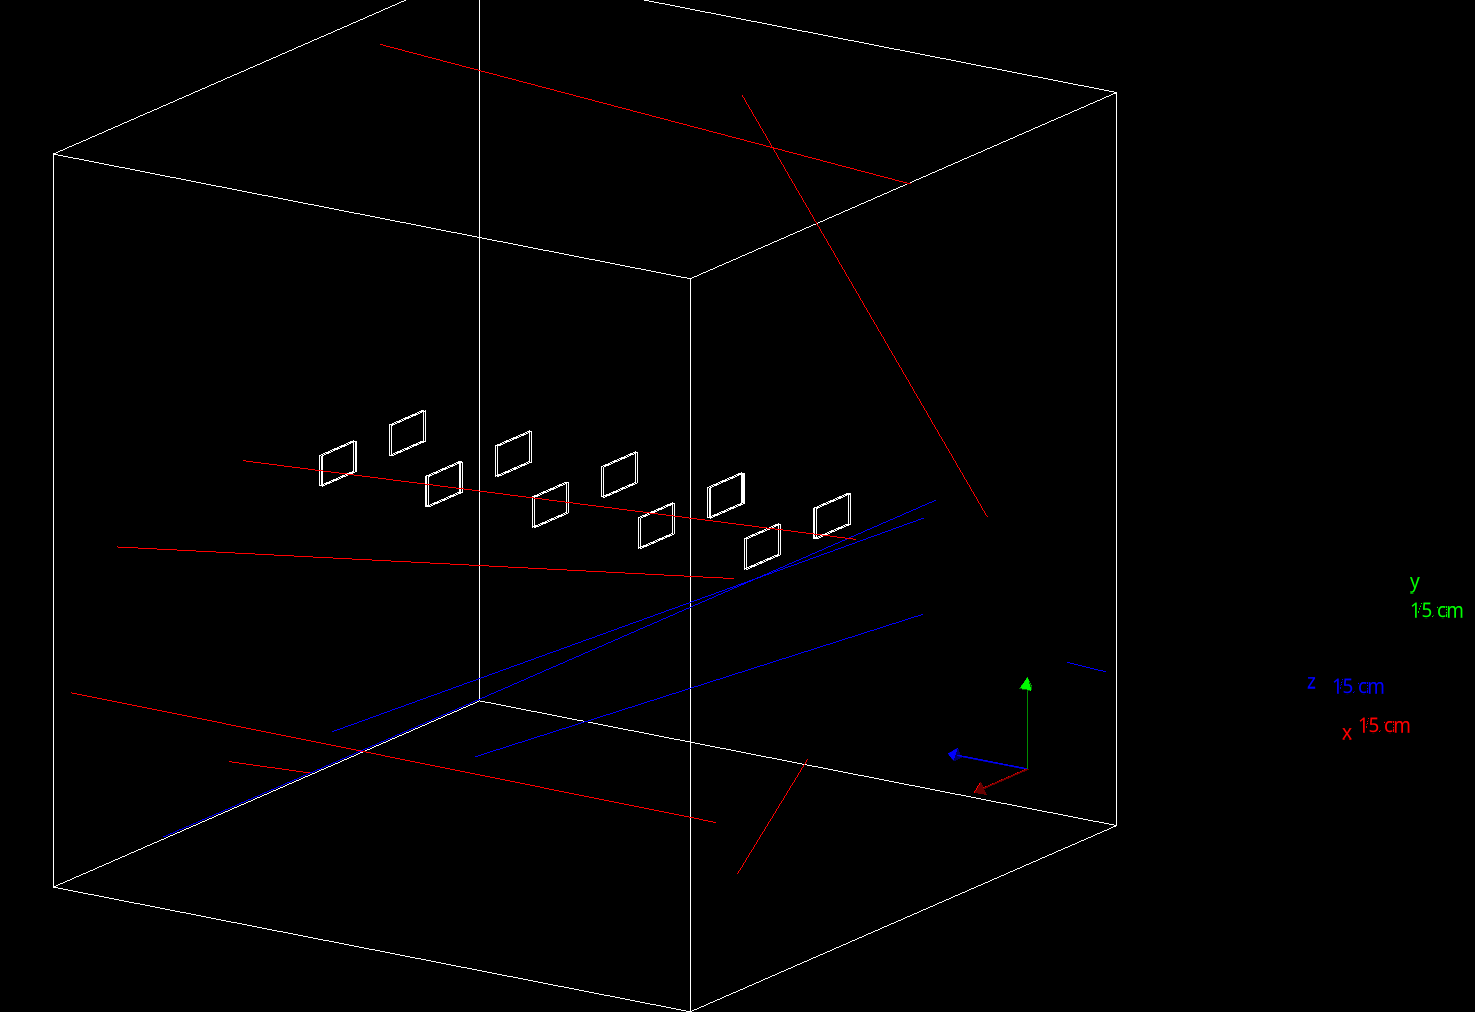
\includegraphics[width=0.48\textwidth]{img/detector.png}
    \caption{Geometry of the modules in the cryostat. The particles are impinging along the +z axis (blue in the figure)}
    \label{fig:Detector}
\end{figure}

\section{Pipeline of the development}
This project was developed entirely in C++, and many tools and libraries were used:
\begin{itemize}
    \item \textbf{Geant4}: Framework used to simulate the interaction of particles in the detector
    \item \textbf{ROOT}: Framework used to manage the data and perform the track reconstruction 
    \item \textbf{CMake}: Used to automate the generation of the makefile across different systems
    \item \textbf{CCache} (Optional): Used to speed up recompilation by caching previous compilations and detecting when the same compilation is being done again.
    \item \textbf{Catch2}: Library to perform Unit-Testing
    \item \textbf{cppcheck}: Static analysis tool 
    \item \textbf{Doxygen}: Used to generate the documentation from the source code
    \item \textbf{Github-Action}: Used to automatically build and deploy the documentation on github-pages
    \item \textbf{cppitertools}: Library to exploit python-like enumerate loops.
    \end{itemize}
\\
Due to the significant size of the dependencies (Geant4 and ROOT), the continuous integration was not implemented because it is impossible to build them at each runner's start.
3 strategies could be implemented to be able to perform the continuous integration:
\begin{enumerate}
    \item \textbf{Self-hosted runners}: Instead of using the machines provided by Github (or any other host), a self-hosted machine (with the dependencies installed) can be used.\\
    This solution was not implemented due to security issues (A simple pull request can run  malicious code on the machine)
    \item \textbf{Static Linking}: Dependencies can be statically linked to the binaries. This method does not solve the continuous integration problem. The binaries have to be built locally before git-pushing, and the runners can only execute them. \\
    Furthermore, the binaries will be very large.
    \item \textbf{Docker Container}: We can create a docker container that contains all the dependencies, so the runner has only to load the container and run the continuous integration in it.\\
    This is the most convenient solution, but, unluckily, the size of the container will be probably larger than a guaranteed space for a free account (500MB)
\end{enumerate}
Due to these issues, compiling and tests were run only on local machines.

\section{Simulation}
Geant4 is a toolkit for simulating the passage of particles through matter.
\\
Geant provides many base abstract classes, and the user has to create concrete classes that inherit from these and implement their virtual methods.
\\
All the parameters of the simulation (physical parameters, geometric parameters, trigger parameters, file paths, etc.) were grouped into namespaces in a single header file (UserParameters.hh), so if the user wants to try different configurations, they can do it by editing just one file.

\subsection{Physics}
In Geant, the user has to manually define the particles and physical processes involved in the simulation.
\\
The abstract class G4VModularPhysicsList provides some standard Physics modules. In this simulation, the module G4EmStandardPhysics was used.
\\
It defines:
\begin{itemize}
    \item Compton scattering, photoelectric effect, and pair production for photons
    \item ionization, bremsstrahlung and multiple scattering for $e^+$, $e^-$ and muons
    \item positron annihilation
    \item pair production by muons
\end{itemize}
To avoid infrared divergences that lead to the production of a lot of low-energy delta rays, a range cut was set (10 cm in air, 0.1mm in silicon).

\subsection{Particle Gun}
\label{ssec:PG}
The particles generated by the particle gun are $\mu^+$ and $\mu^-$ generated uniformly on a face of the world box and shot along the +z axis according to:
\begin{itemize} 
    \item The muon charge distribution at the sea surface ($\frac{\mu^+}{\mu^-}=1.3$).
    \item The angular distribution of cosmic rays at the sea surface $\cos^2(\theta)$
    \item The energy distribution of cosmic rays at the sea surface between 1 GeV and 1 TeV
    \\
    $ \frac{dN_{\mu}}{dE_{\mu} d \Omega} \approx \frac{0.14 E_{\mu}^{-2.7}}{cm^2 \; s \;sr \; GeV} \left( \frac{1}{1+\frac{1.1 E_{\mu}\cos{\theta}}{115 GeV}} + \frac{0.054}{1+\frac{1.1 E_{\mu}\cos{\theta}}{850 GeV}} \right) $
\end{itemize}
These variables are generated using the GetRandom method of the ROOT::TF1 class.
\\
Most of the generated particles do not pass through the detector because the world box is much larger than the detector (the detector is 30 cm x 5 cm x 80 cm, while the world box is 120 cm x 120 cm x 120 cm).
\\
If the world box is smaller, then the tail of the reconstructed angular distribution is suppressed.
The most efficient solution would be to convolve the distribution of the parameters of the particles with the geometric acceptance of the detector, but due to the simplicity of the simulation, a brute force approach was preferred, and to obtain more hits, we just generated more particles.
\subsection{Read Out}
In Geant is possible to define a read-out geometry in parallel to the real geometry of the detector by exploiting abstract classes like G4VReadOutGeometry. Unfortunately, the documentation about these classes is practically inexistent, so a simple ReadOut class was implemented.
\\
Given the position of the modules in the world box and the number and dimension of the strip and pixels, it provides a method that can transform the real position of a hit into the position of the center of the channel that was hit.
\\
To accomplish this task, the algorithm is as follows:
\begin{enumerate}
    \item find the position of the closest module to the hit on a given axis
    \item translates the hit position in the frame of the module
    \item calculate the position of the center of the channel that was hit in the module frame
    \item translates back to the world frame
\end{enumerate}
This is applied to the 3 axes separately.


\subsection{Trigger}
The trigger implemented is very simple:
\begin{itemize}
    \item \textbf{Pulse height discrimination:} Rejects all hits with released energy below a given threshold (40 keV).
    \\
    The main scope of the pulse height discrimination is to limit the presence of delta rays' hits in the data.
    \item \textbf{Coincidence}: Accept only events with hits in at least two different PS module layers.
\end{itemize}

\subsection{Event data structure}
The data are saved in a root file. The TFile has one TTree with a branch in which a custom Event object is saved.
The structure of the Event class is the following:
\dirtree{%
.0 Event.
.1 eventID.
.1 detectorData.
.2 TrackID.
.2 ParticleID (0 $\mu^-$,1 $\mu^+$,2 $e^-$,3 $e^+$,4 $\gamma$).
.2 EnergyDeposited (keV) .
.2 posX (position of the channel hit in mm).
.2 posY.
.2 posZ.
.2 Layer (odds are pixels, evens are strips).
.1 truthBeamData.
.2 posX (position of the particle gun).
.2 posY.
.2 posZ.
.2 phi (polar angle).
.2 theta (azimuthal angle).
.2 energy (GeV).
.2 particleID (0 $\mu^-$, 1 $\mu^+$).
}.
\newline
The Event object contains a DetectorData and a TruthBeamData object.\\
The Detector data objects contain std vectors filled with data from hits in the detector, while the TruthBeamDataObject contains the data of the beam generated by the particle gun.

\subsection{Data management and multithreading}
Geant4 provides the class G4VAnalysisManager, a thread-safe wrapper for some simple ROOT classes and methods.\\
It creates a different file for each worker thread so the threads can work in parallel on different data avoiding any conflict due to data races.
\\
Unfortunately, the G4VAnalysisManager is very inconvenient to use to create and manipulate trees and custom objects, so a DataManager and DataManagerMT classes were created to manage the TFiles, and ROOT was used to fill them with the Event objects.
\\
\\
In Geant, the singleton is the most used design pattern for sharing objects among different classes.
\\
Leaving aside the considerations about this choice, the real pain about singletons comes when they have to deal with thread safety, but for consistency, also DataManager and DataManagerMT are singletons.
\\
\\
DataManager is a singleton that contains a TFile, a TTree, and an Event class object.
The strategy to maintain thread safety is the same as Geant: each thread works on a different file. Nevertheless, DataManager is a singleton, so we cannot have multiple TFile. For this reason, we defined DataManagerMT as a friend class of DataManager.
\\
The role of DataManagerMT is to create an std vector containing multiple instances (one each thread)
 of DataManager (it can do it because it is a friend class of DataManager so it can call the private constructor).
 \\
 \\
 At the beginning of the run, the master thread creates the DataManagerMT instance, and then each worker thread gets the pointer to the DataManagerMT object that allows it to get the pointer to its own DataManager object.
 In this way, thread safety is accomplished.

\subsection{Results}
At the end of the simulation, 500.000 particles were generated, and the trigger saved 1819 events.\\
The big difference between these two numbers is due to different reasons:
\begin{itemize}
    \item The dimension of the world box (discussed in subsection \hyperref[ssec:PG]{Particle Gun})
    \item The large energy threshold set (40keV)
\end{itemize}

The root file containing the results is output.root. It is in the \href{https://github.com/pviscone/TrackG4/tree/main/data}{data folder of the repo}
In fig \ref{fig:energy} and fig \ref{fig:posX} there are shown as an example the energy deposited in the detector and the x coordinate of the channel that was hit.


\section{Track reconstruction}
To reconstruct the tracks, a simple toy model was used to fit two straight lines in the XZ and YZ projection planes.
\\
The initial parameter of the fit is computed simply by sorting the hits along the z-axis and computing the linear function's two parameters, considering only the first and the last point.\\
Then the fit is performed using the TGraphError class, considering as error bar the pitch of pixels/strips divided by $\sqrt{12}$.
\\
\\
Despite the trigger in the simulation, delta rays' hits are still present.
\\
\subsection{Structure of the data}
The root file containing the results of the fit is made up a simple NTuple structured as follows:
\dirtree{%
.1 fitResults.
.2 evID (Id of the reconstructed event).
.2 nHit (num of hits). 
.2 x0.
.2 x0\_err.
.2 mx.
.2 mx\_err.
.2 chi2zx (reduced chi2 of the ZX fit).
.2 y0.
.2 y0\_err.
.2 my.
.2 my\_err.
.2 chi2zy.
}.
\\
The fitted functions are $z=m_x x+x_0$ and $z=m_y y +y_0$ in the frame of the world box.\\
The length units are millimetres.
\\
\\
The fit\_results.root file and the plots of the fits are stored in the \href{https://github.com/pviscone/TrackG4/tree/main/data}{data folder of the repo}
\\
\\
For example, in fig \ref{fig:mx}, fig \ref{fig:x0} there are shown the best-fit parameters in the XZ projection.
In fig\refFig shown ths plot of a well-fitted event, while in fig\ref{fig:bad} is shown the plot of an event affected by the presence of delta rays.
%----------------------------------------------------------------------------------------
%	BIBLIOGRAPHY
%----------------------------------------------------------------------------------------
\section{Conclusion}
In conclusion, this is just a basic simulation, but it could be a good starting point to develop more complex simulations accounting for other aspects of the detector (efficiency, radiation hardness, etc.) to characterize the PS modules prototypes of the future CMS outer tracker.

\printbibliography[title={Bibliography}] % Print the bibliography, section title in curly brackets

\onecolumn

\section*{Images}
\subsection*{Simulation}

\begin{figure}[h!]
    \centering
    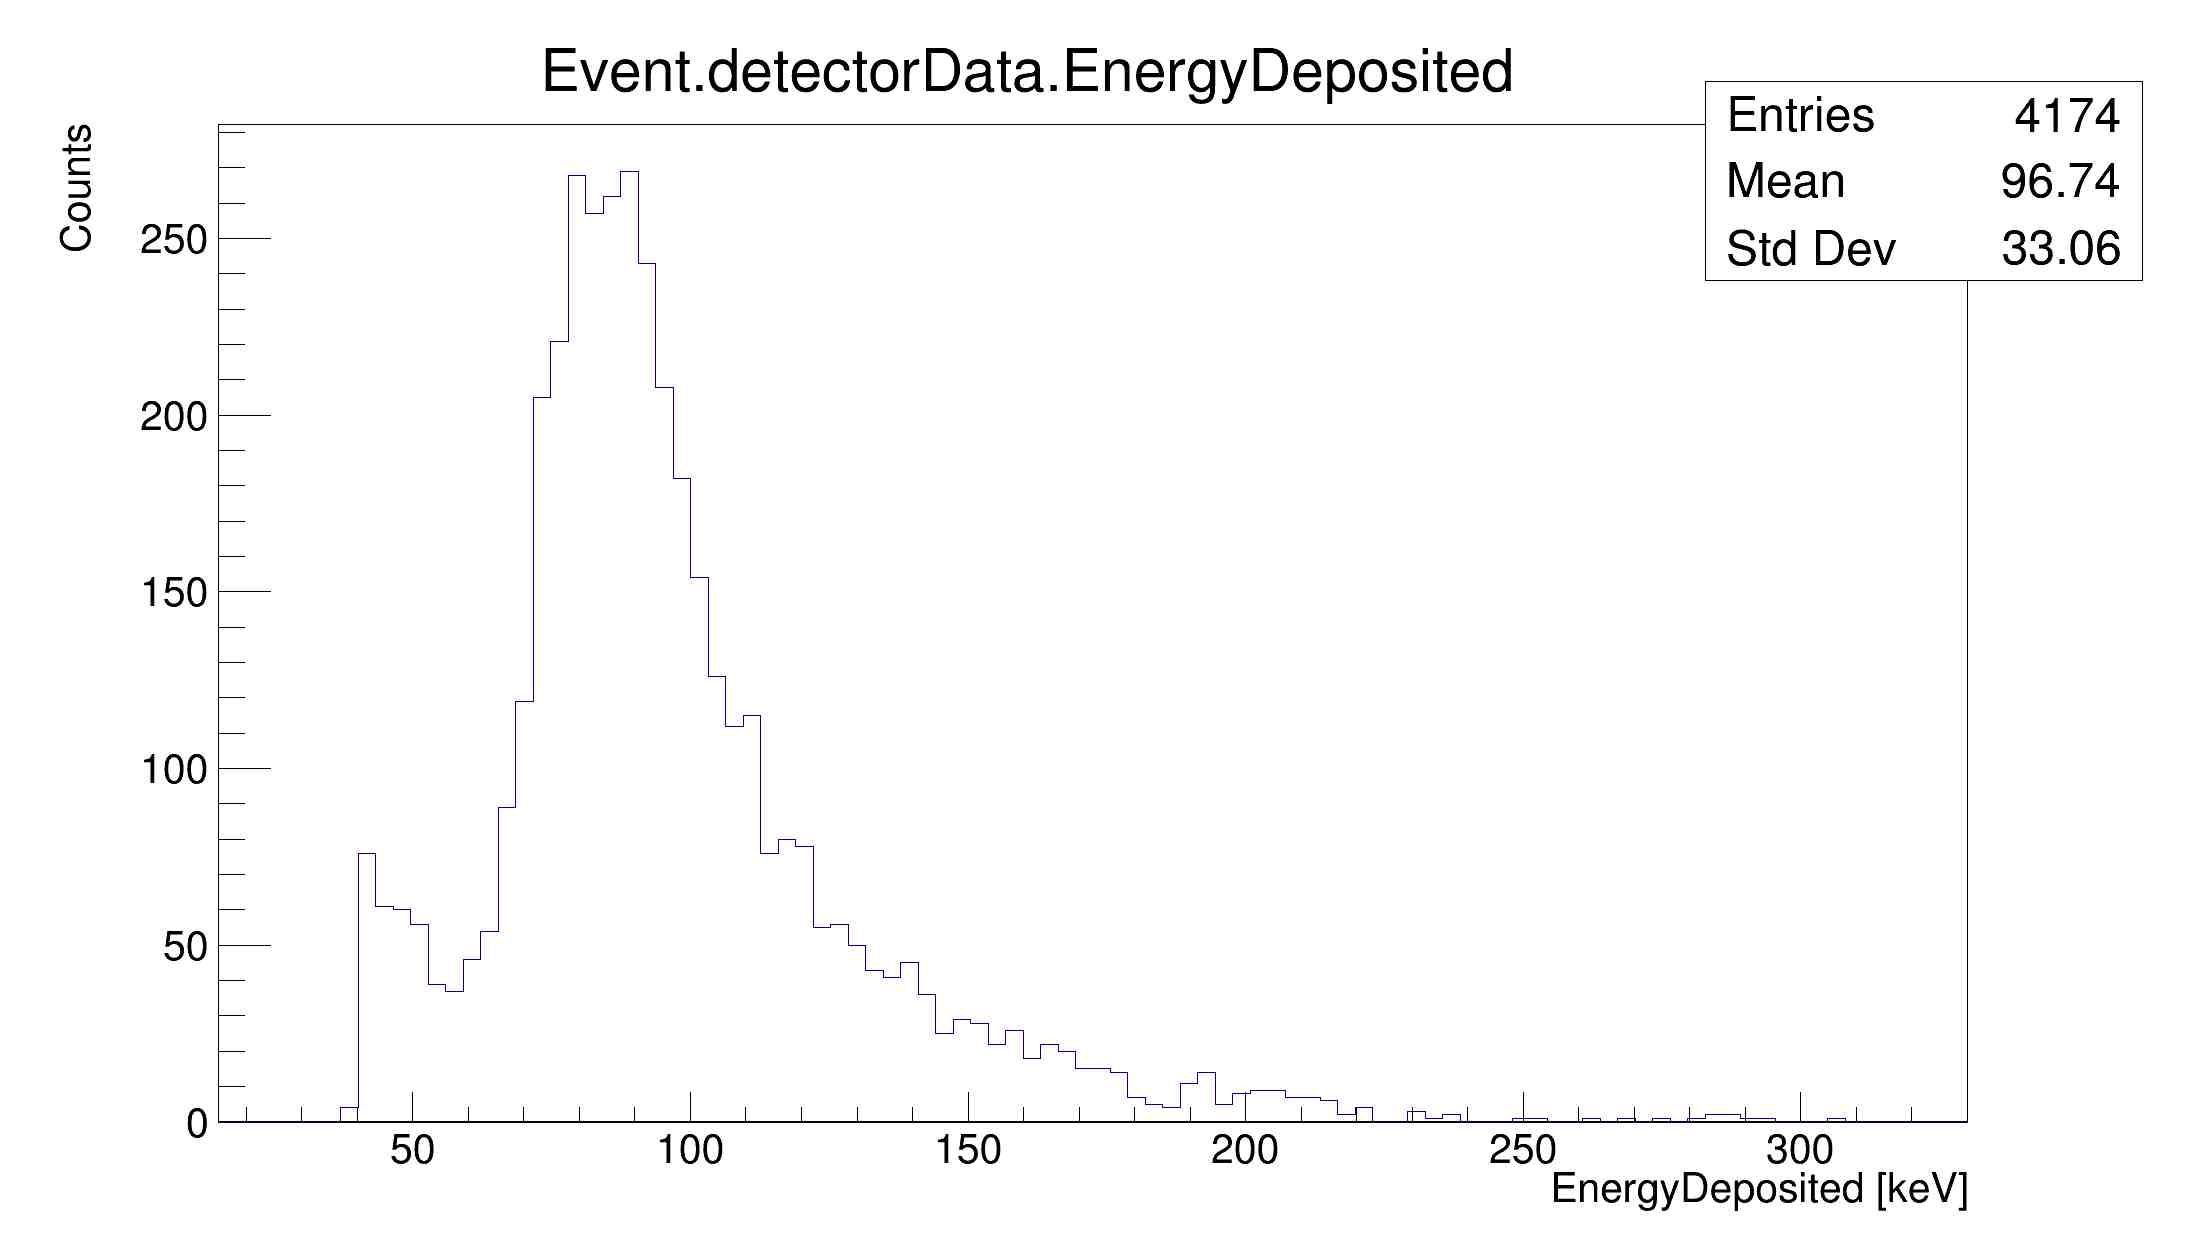
\includegraphics[width=0.8 \textwidth]{img/energy.jpg}
    \caption{Energy released in the detector by each hit. The cut at 40 keV is due to the energy threshold set}.
    \label{fig:energy}
\end{figure}
    
\begin{figure}[h!]
    \centering
    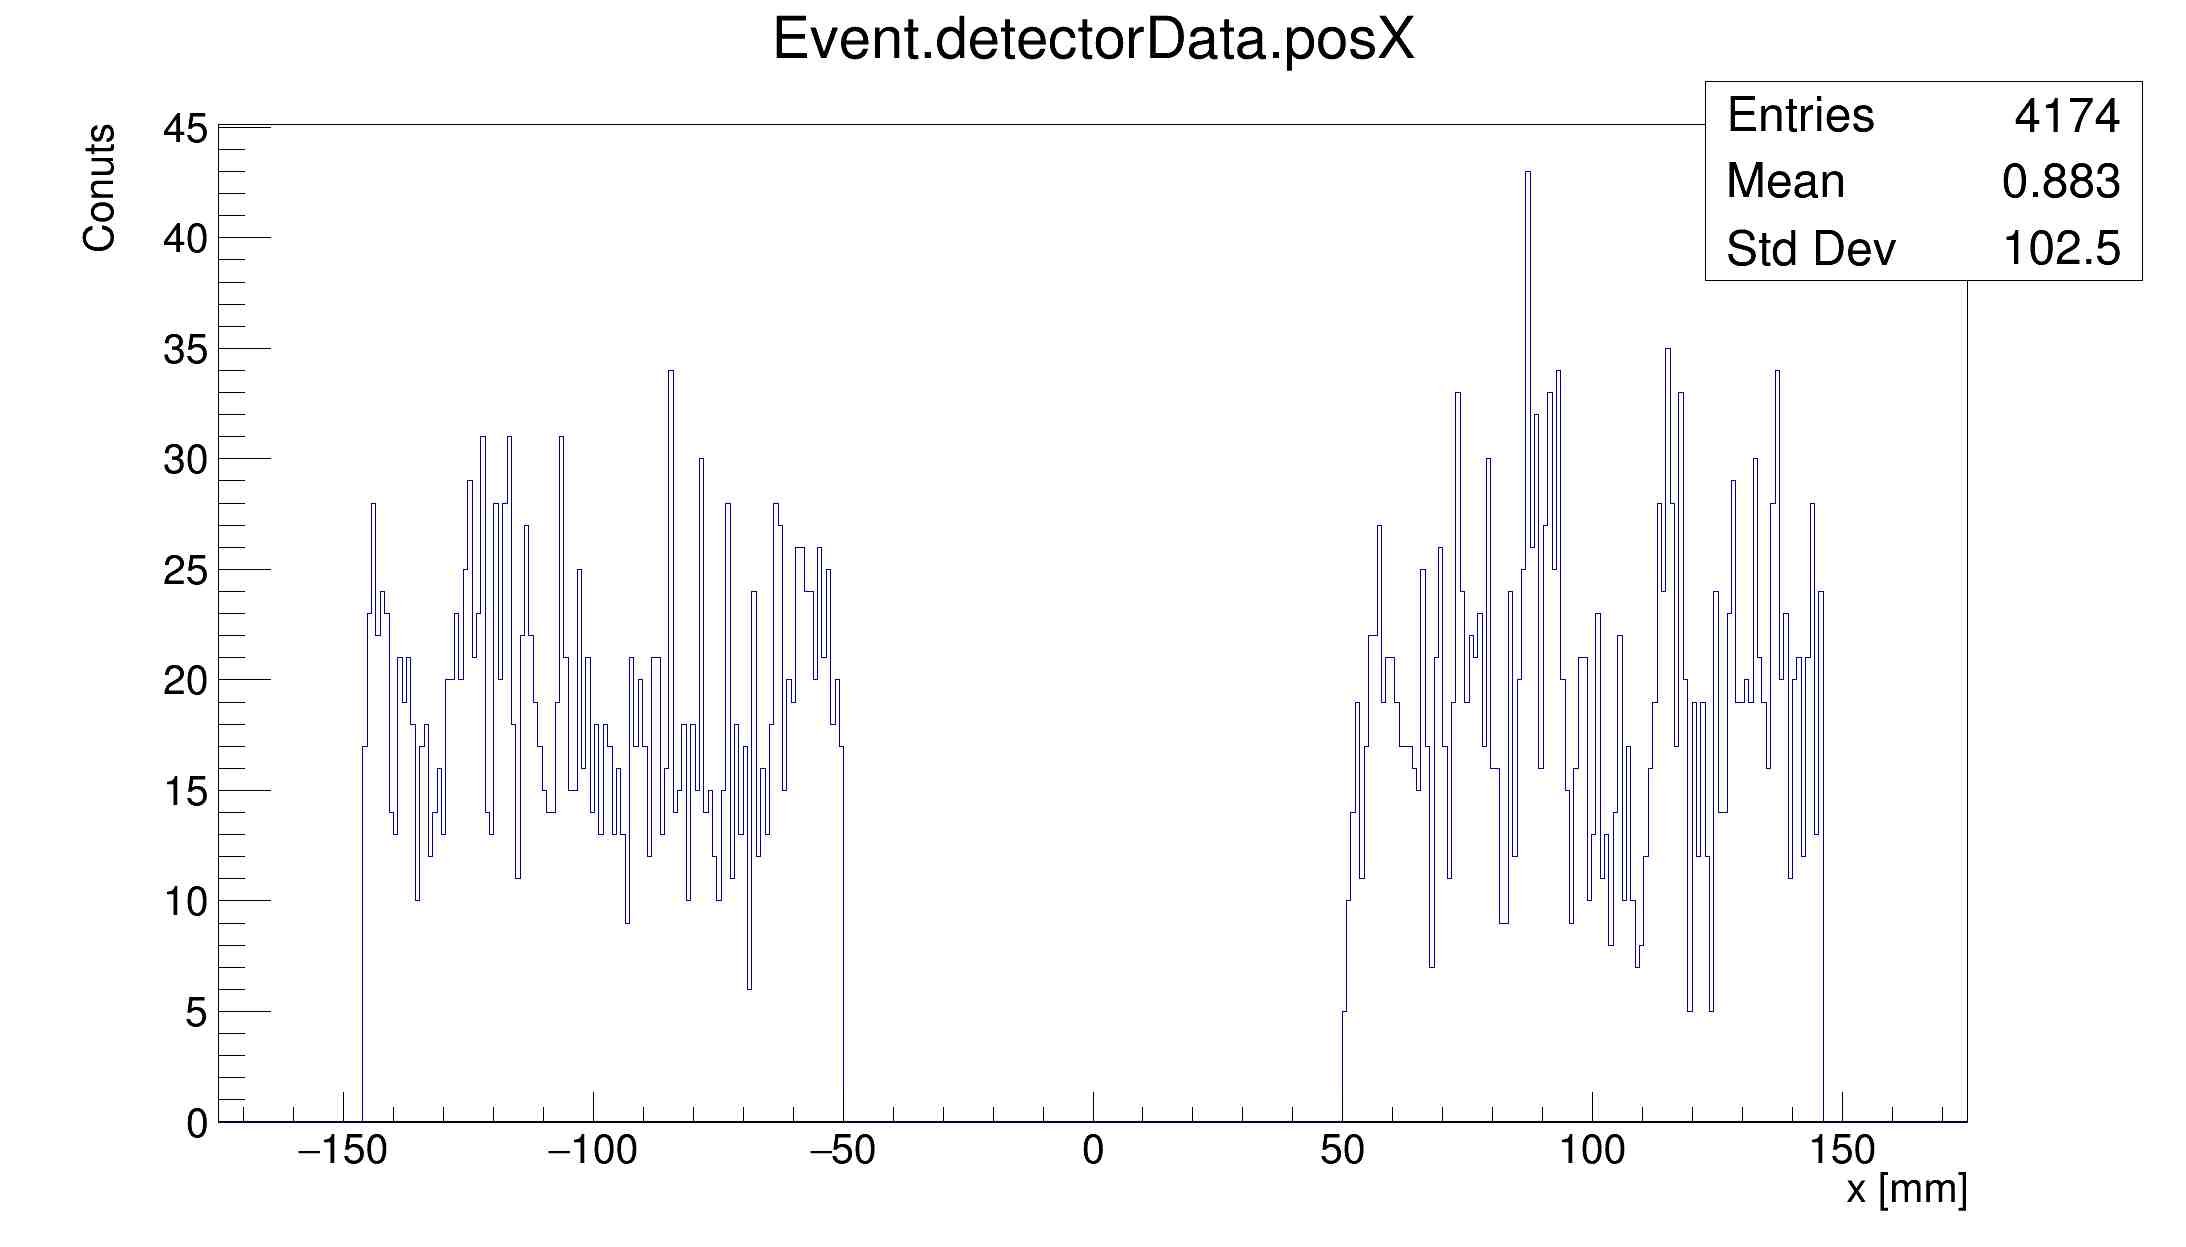
\includegraphics[width=0.8 \textwidth]{img/posx.jpg}
    \caption{Position of the hits along the x-axis}
    \label{fig:posX}
\end{figure}
\newpage
\subsection{Fit}

\begin{figure}[h!]
    \centering
    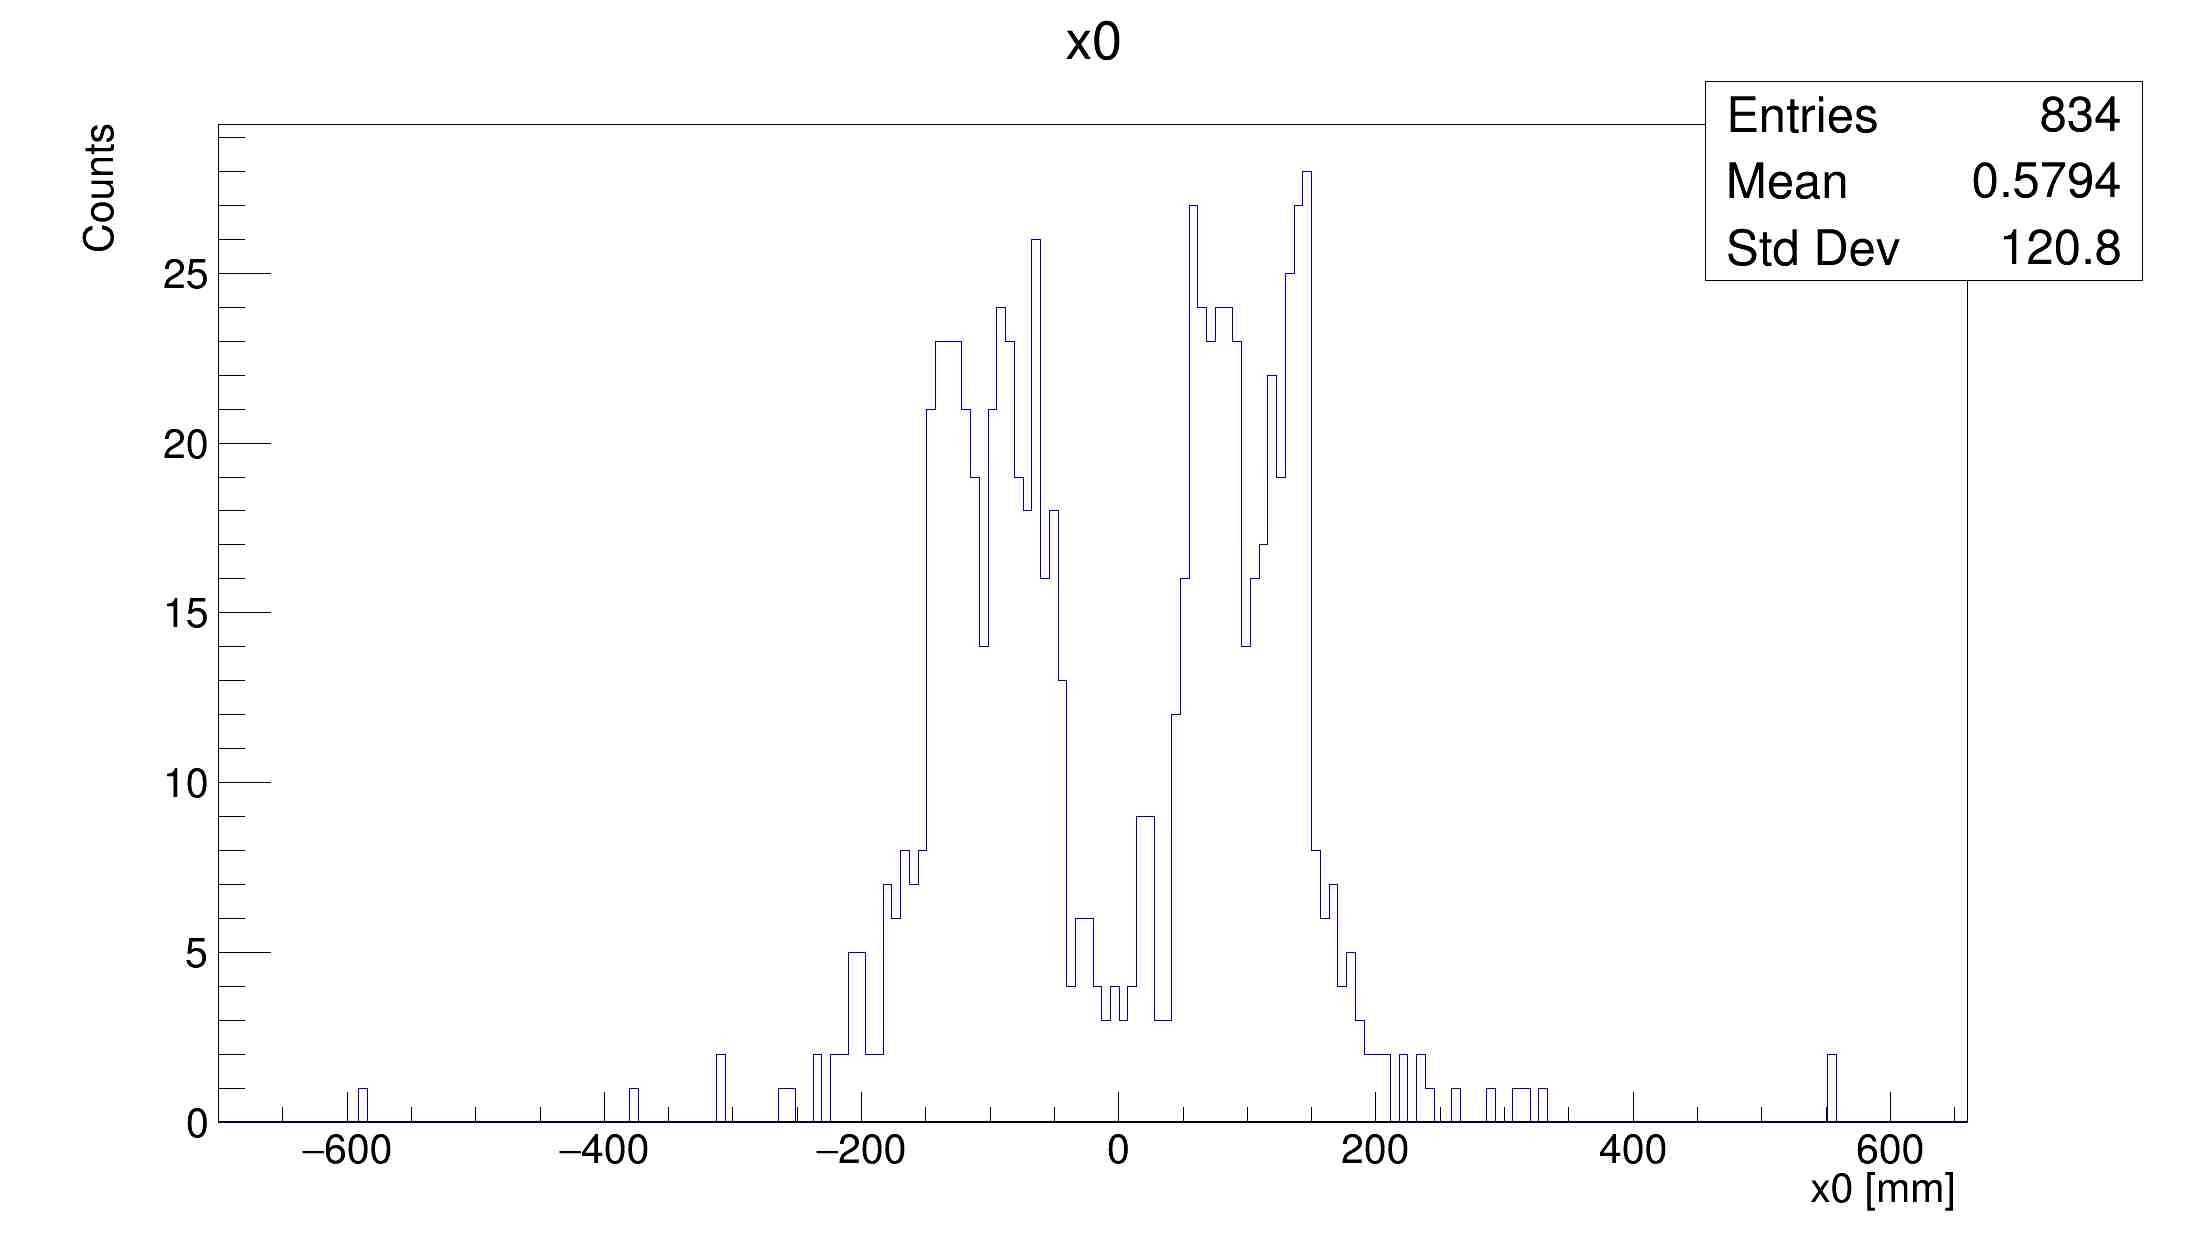
\includegraphics[width=0.8 \textwidth]{img/x0.jpg}
    \caption{Fitted $x_0$ parameter}
    \label{fig:x0}
\end{figure}

\begin{figure}[h!]
    \centering
    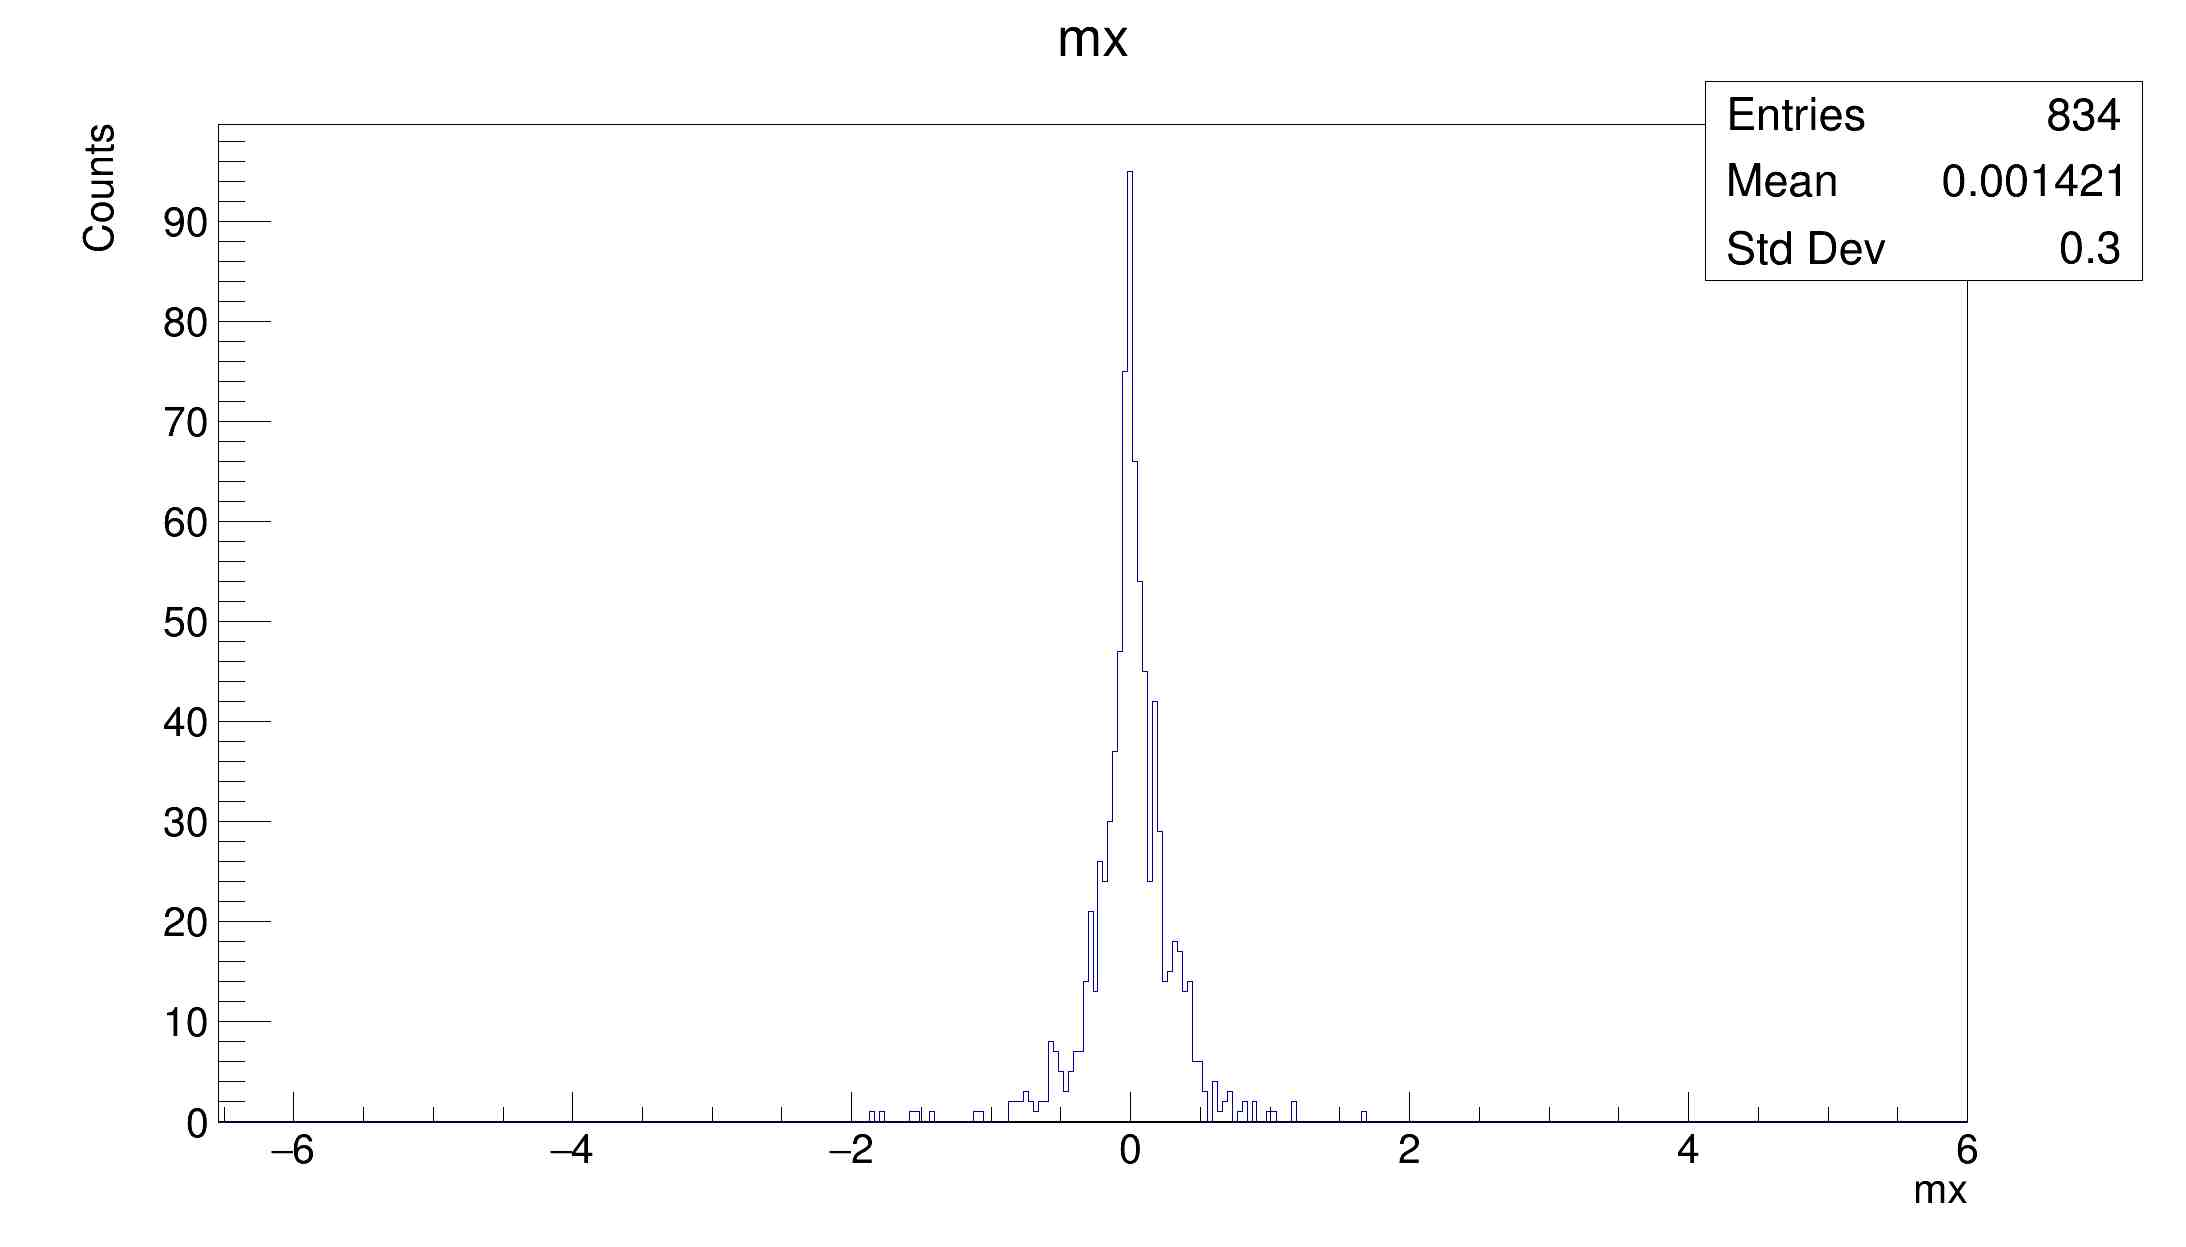
\includegraphics[width=0.8 \textwidth]{img/mx.jpg}
    \caption{Fitted $m_x$ parameter}
    \label{fig:mx}
\end{figure}

\onecolumn
\begin{figure}[h!]
    \centering
    \subfigure[]{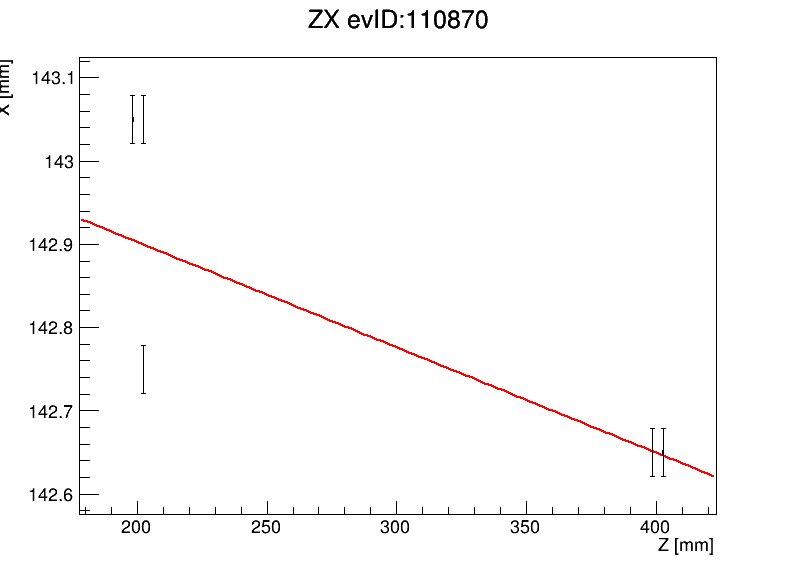
\includegraphics[width=0.48 \textwidth]{img/zx_110870.png}}
    \subfigure[]{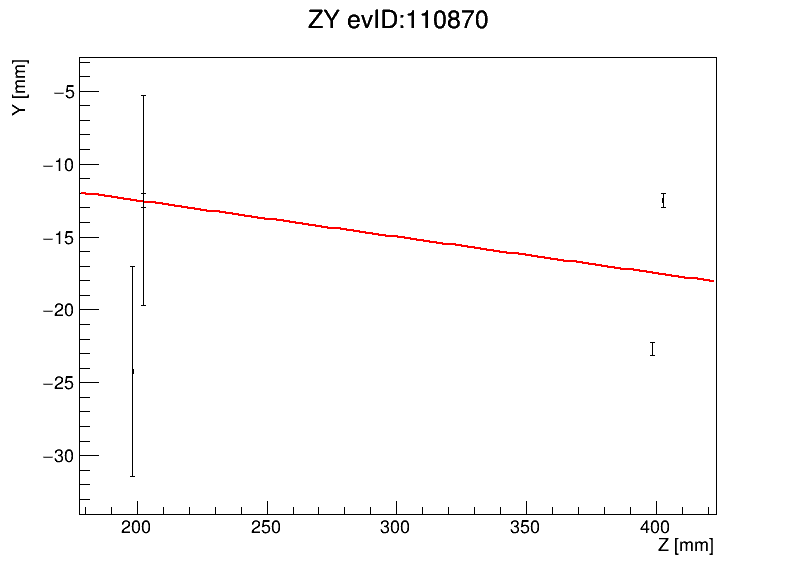
\includegraphics[width=0.48 \textwidth]{img/zy_110870.png}}
    \caption{Event affected by the presence of delta rays' hits}
    \label{fig:bad}
\end{figure}

\begin{figure}[h!]
    \centering
    \subfigure[]{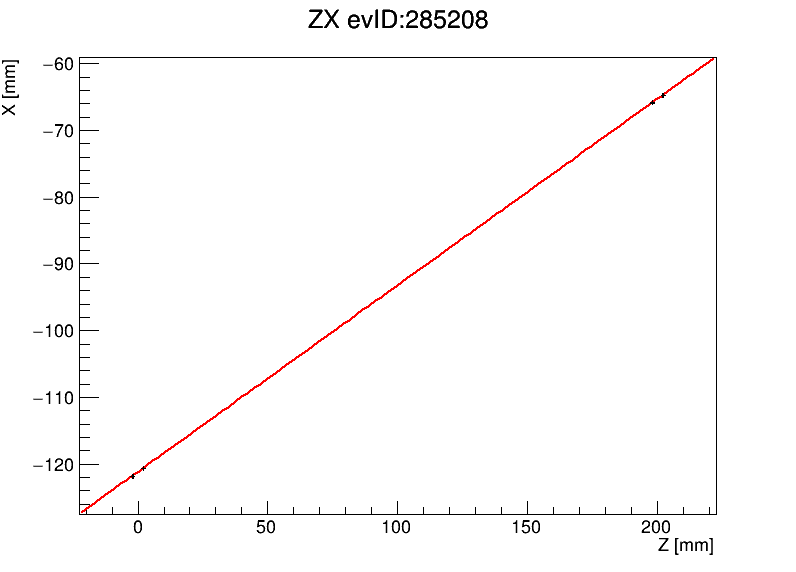
\includegraphics[width=0.48 \textwidth]{img/zx_285208.png}}
    \subfigure[]{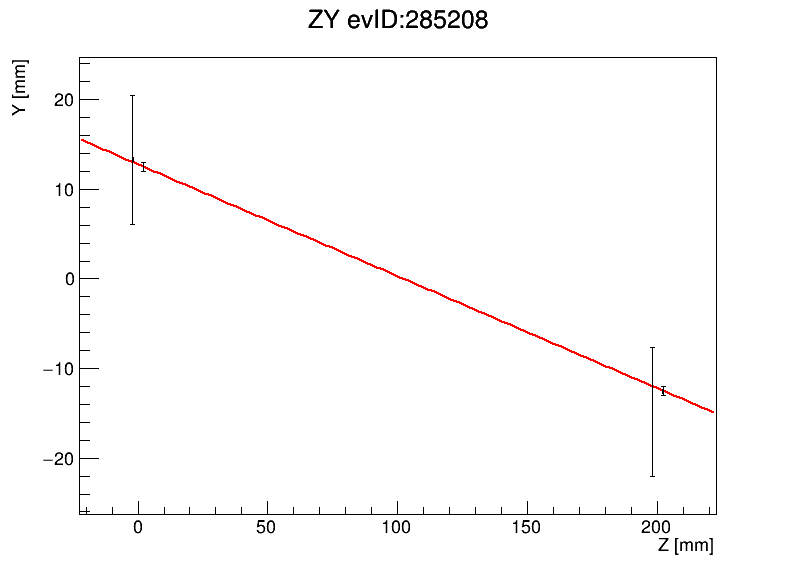
\includegraphics[width=0.48 \textwidth]{img/zy_285208.png}}
    \caption{Well fitted event. Multiple scattering clearly visible}
    \label{fig:well}
\end{figure}



%----------------------------------------------------------------------------------------

\end{document}
\